\begin{frame}{Limit Orders}
  Each participant maintains a set of \textbf{limit orders}, which the exchange uses 
  to automatically infer whether they would agree to any hypothetical trade or not.\\
  Here is what a limit order may look like:
  \begin{sqt:tip}
    Alice tells the exchange
    \begin{center}
      ``I am willing to sell a maximum of 5 AAPL shares.\\
      I am willing to sell each share at a price of \$30 or better.''
    \end{center}
  \end{sqt:tip}

  This is called \textbf{inserting} an order.

  \begin{center}
    \input{assets/limit_order_intro.tex}
  \end{center}
\end{frame}

\begin{frame}{Bids and Offers}
  By submitting the \textbf{sell order}, Alice authorizes the exchange to accept trades on her behalf, 
  until 5 AAPL shares have been \textbf{sold}. Once this happens, the order is considered \textbf{filled}.

  \begin{sqt:definition}
    \begin{itemize}
      \item A \textbf{bid} (buy order) expresses a willingness to buy
      \item An \textbf{offer/ask} (sell order) expresses a willingness to sell
    \end{itemize}
  \end{sqt:definition}

  \begin{center}
    

\tikzset{every picture/.style={line width=0.75pt}} %set default line width to 0.75pt        

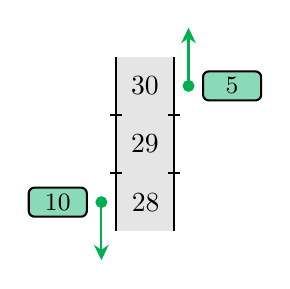
\begin{tikzpicture}[x=0.75pt,y=0.75pt,yscale=-0.7,xscale=0.7]
%uncomment if require: \path (0,300); %set diagram left start at 0, and has height of 300

%Shape: Rectangle [id:dp13563874266693043] 
\draw  [draw opacity=0][fill={rgb, 255:red, 0; green, 0; blue, 0 }  ,fill opacity=0.1 ] (230,100) -- (270,100) -- (270,220) -- (230,220) -- cycle ;
%Rounded Rect [id:dp5561959472232012] 
\draw  [fill={rgb, 255:red, 138; green, 218; blue, 184 }  ,fill opacity=1 ][line width=0.75]  (290,114) .. controls (290,111.79) and (291.79,110) .. (294,110) -- (326,110) .. controls (328.21,110) and (330,111.79) .. (330,114) -- (330,126) .. controls (330,128.21) and (328.21,130) .. (326,130) -- (294,130) .. controls (291.79,130) and (290,128.21) .. (290,126) -- cycle ;
%Straight Lines [id:da05571726881476602] 
\draw    (230,100) -- (230,220) (234,140) -- (226,140)(234,180) -- (226,180) ;
%Straight Lines [id:da7319727700794608] 
\draw    (270,100) -- (270,220) (274,140) -- (266,140)(274,180) -- (266,180) ;
%Straight Lines [id:da8116302583311774] 
\draw [color={rgb, 255:red, 0; green, 176; blue, 79 }  ,draw opacity=1 ]   (280,120) -- (280,83) ;
\draw [shift={(280,80)}, rotate = 90] [fill={rgb, 255:red, 0; green, 176; blue, 79 }  ,fill opacity=1 ][line width=0.08]  [draw opacity=0] (10.72,-5.15) -- (0,0) -- (10.72,5.15) -- (7.12,0) -- cycle    ;
\draw [shift={(280,120)}, rotate = 270] [color={rgb, 255:red, 0; green, 176; blue, 79 }  ,draw opacity=1 ][fill={rgb, 255:red, 0; green, 176; blue, 79 }  ,fill opacity=1 ][line width=0.75]      (0, 0) circle [x radius= 3.35, y radius= 3.35]   ;
%Rounded Rect [id:dp9565192834046984] 
\draw  [fill={rgb, 255:red, 138; green, 218; blue, 184 }  ,fill opacity=1 ][line width=0.75]  (170,194) .. controls (170,191.79) and (171.79,190) .. (174,190) -- (206,190) .. controls (208.21,190) and (210,191.79) .. (210,194) -- (210,206) .. controls (210,208.21) and (208.21,210) .. (206,210) -- (174,210) .. controls (171.79,210) and (170,208.21) .. (170,206) -- cycle ;
%Straight Lines [id:da8103839365180321] 
\draw [color={rgb, 255:red, 0; green, 176; blue, 79 }  ,draw opacity=1 ]   (220,200) -- (220,237) ;
\draw [shift={(220,240)}, rotate = 270] [fill={rgb, 255:red, 0; green, 176; blue, 79 }  ,fill opacity=1 ][line width=0.08]  [draw opacity=0] (10.72,-5.15) -- (0,0) -- (10.72,5.15) -- (7.12,0) -- cycle    ;
\draw [shift={(220,200)}, rotate = 90] [color={rgb, 255:red, 0; green, 176; blue, 79 }  ,draw opacity=1 ][fill={rgb, 255:red, 0; green, 176; blue, 79 }  ,fill opacity=1 ][line width=0.75]      (0, 0) circle [x radius= 3.35, y radius= 3.35]   ;

% Text Node
\draw (250,119.5) node    {$30$};
% Text Node
\draw (310,120) node  [font=\small]  {${\textstyle 5}$};
% Text Node
\draw (250,160) node    {$29$};
% Text Node
\draw (250.5,200) node    {$28$};
% Text Node
\draw (190,200) node  [font=\small]  {$10$};


\end{tikzpicture}

  \end{center}
\end{frame}

\begin{frame}{Orderbook}
  \begin{sqt:definition}
    The exchange keeps track of each participant's \textbf{open orders} (unfilled),\\
    and collects them into an \textbf{orderbook}.
  \end{sqt:definition}

  \begin{center}
    \input{assets/orderbook.tex}
  \end{center}
\end{frame}

\begin{frame}{Limit Orders In Cross}

  \begin{sqt:definition}
    Two limit orders are \textbf{in cross} if
    \begin{itemize}
      \item One order is a \textbf{bid} and the other is an \textbf{ask}.
      \item There exists an \textbf{intersection} between the price ranges they are willing to trade at
    \end{itemize}
  \end{sqt:definition}
  \begin{center}
    

\tikzset{every picture/.style={line width=0.75pt}} %set default line width to 0.75pt        

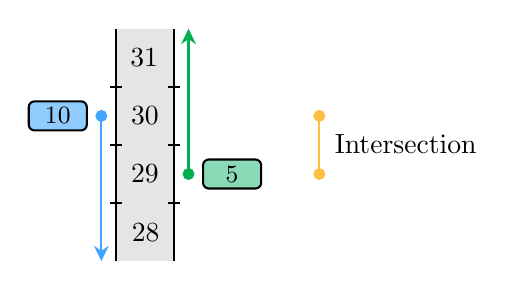
\begin{tikzpicture}[x=0.75pt,y=0.75pt,yscale=-0.7,xscale=0.7]
%uncomment if require: \path (0,300); %set diagram left start at 0, and has height of 300

%Shape: Rectangle [id:dp13563874266693043] 
\draw  [draw opacity=0][fill={rgb, 255:red, 0; green, 0; blue, 0 }  ,fill opacity=0.1 ] (230,60) -- (270,60) -- (270,220) -- (230,220) -- cycle ;
%Rounded Rect [id:dp5561959472232012] 
\draw  [fill={rgb, 255:red, 138; green, 218; blue, 184 }  ,fill opacity=1 ][line width=0.75]  (290,154) .. controls (290,151.79) and (291.79,150) .. (294,150) -- (326,150) .. controls (328.21,150) and (330,151.79) .. (330,154) -- (330,166) .. controls (330,168.21) and (328.21,170) .. (326,170) -- (294,170) .. controls (291.79,170) and (290,168.21) .. (290,166) -- cycle ;
%Straight Lines [id:da05571726881476602] 
\draw    (230,60) -- (230,220) (234,100) -- (226,100)(234,140) -- (226,140)(234,180) -- (226,180) ;
%Straight Lines [id:da7319727700794608] 
\draw    (270,60) -- (270,220) (274,100) -- (266,100)(274,140) -- (266,140)(274,180) -- (266,180) ;
%Straight Lines [id:da8116302583311774] 
\draw [color={rgb, 255:red, 0; green, 176; blue, 79 }  ,draw opacity=1 ]   (280,160) -- (280,63) ;
\draw [shift={(280,60)}, rotate = 90] [fill={rgb, 255:red, 0; green, 176; blue, 79 }  ,fill opacity=1 ][line width=0.08]  [draw opacity=0] (10.72,-5.15) -- (0,0) -- (10.72,5.15) -- (7.12,0) -- cycle    ;
\draw [shift={(280,160)}, rotate = 270] [color={rgb, 255:red, 0; green, 176; blue, 79 }  ,draw opacity=1 ][fill={rgb, 255:red, 0; green, 176; blue, 79 }  ,fill opacity=1 ][line width=0.75]      (0, 0) circle [x radius= 3.35, y radius= 3.35]   ;
%Straight Lines [id:da8103839365180321] 
\draw [color={rgb, 255:red, 65; green, 165; blue, 255 }  ,draw opacity=1 ]   (220,120) -- (220,217) ;
\draw [shift={(220,220)}, rotate = 270] [fill={rgb, 255:red, 65; green, 165; blue, 255 }  ,fill opacity=1 ][line width=0.08]  [draw opacity=0] (10.72,-5.15) -- (0,0) -- (10.72,5.15) -- (7.12,0) -- cycle    ;
\draw [shift={(220,120)}, rotate = 90] [color={rgb, 255:red, 65; green, 165; blue, 255 }  ,draw opacity=1 ][fill={rgb, 255:red, 65; green, 165; blue, 255 }  ,fill opacity=1 ][line width=0.75]      (0, 0) circle [x radius= 3.35, y radius= 3.35]   ;
%Rounded Rect [id:dp6586100738433943] 
\draw  [fill={rgb, 255:red, 143; green, 203; blue, 253 }  ,fill opacity=1 ][line width=0.75]  (170,114) .. controls (170,111.79) and (171.79,110) .. (174,110) -- (206,110) .. controls (208.21,110) and (210,111.79) .. (210,114) -- (210,126) .. controls (210,128.21) and (208.21,130) .. (206,130) -- (174,130) .. controls (171.79,130) and (170,128.21) .. (170,126) -- cycle ;
%Straight Lines [id:da4565659656057395] 
\draw [color={rgb, 255:red, 255; green, 191; blue, 65 }  ,draw opacity=1 ]   (370,120) -- (370,160) ;
\draw [shift={(370,160)}, rotate = 90] [color={rgb, 255:red, 255; green, 191; blue, 65 }  ,draw opacity=1 ][fill={rgb, 255:red, 255; green, 191; blue, 65 }  ,fill opacity=1 ][line width=0.75]      (0, 0) circle [x radius= 3.35, y radius= 3.35]   ;
\draw [shift={(370,120)}, rotate = 90] [color={rgb, 255:red, 255; green, 191; blue, 65 }  ,draw opacity=1 ][fill={rgb, 255:red, 255; green, 191; blue, 65 }  ,fill opacity=1 ][line width=0.75]      (0, 0) circle [x radius= 3.35, y radius= 3.35]   ;

% Text Node
\draw (250,119.5) node    {$30$};
% Text Node
\draw (310,160) node  [font=\small]  {${\textstyle 5}$};
% Text Node
\draw (250,160) node    {$29$};
% Text Node
\draw (250.5,200) node    {$28$};
% Text Node
\draw (249.5,80) node    {$31$};
% Text Node
\draw (190,120) node  [font=\small]  {$10$};
% Text Node
\draw (429.5,139.5) node   [align=left] {Intersection};


\end{tikzpicture}

  \end{center}
\end{frame}

\begin{frame}{Order Matching Algorithm}
  We will demonstrate \textbf{continuous matching} with \textbf{price-time priority}.\\
  This is a \textbf{matching algorithm} that determines the trades made when orders are inserted.

  \begin{itemize}
    \item Orders are \textbf{received} and then \textbf{handled} by the exchange one at a time.
    \item The order currently being \textbf{handled} is the \textbf{aggressing order}.
    \item The \textbf{aggressing order} is matched against \textbf{open orders} it is \textbf{in cross} with.
    \begin{itemize}
      \item Choose the \textbf{open order} according to \textbf{price-time priority}.
      \item Execute the trade at the price level of the \textbf{open order}, for the maximum quantity possible.
    \end{itemize}
    \item This matching occurs until either:
    \begin{itemize}
      \item The aggressing order runs out of quantity:
      \begin{itemize}
        \item The order is considered \textbf{filled} and is discarded.
      \end{itemize}
      \item No more orders \textbf{in cross} remain:
      \begin{itemize}
        \item The order is \textbf{unfilled} or only \textbf{partially filled}.
        \item If the order was a \textbf{fill-and-kill} (FAK), then the order is discarded.
        \item If the order was a \textbf{good-till-cancel} (GTC), then it is inserted at its price level at the back of the queue.
      \end{itemize}
    \end{itemize}
  \end{itemize}
\end{frame}

\begin{frame}{Small GTC Buy Order: Initial}
  \begin{center}
    \input{assets/small_gtc_frame_0.tex}
  \end{center}
\end{frame}

\begin{frame}{Small GTC Buy Order: Animation}
  \begin{center}
    \only<1>{\input{assets/small_gtc_frame_1.tex}}
    \only<2>{\input{assets/small_gtc_frame_2.tex}}
    \only<3>{\input{assets/small_gtc_frame_3.tex}}
    \only<4>{\input{assets/small_gtc_frame_4.tex}}
    \only<5>{\input{assets/small_gtc_frame_5.tex}}
  \end{center}
\end{frame}

\begin{frame}{Small GTC Buy Order: Result}
  \begin{center}
    \input{assets/small_gtc_frame_result.tex}
  \end{center}
\end{frame}

\begin{frame}{Large GTC Buy Order: Initial}
  \begin{center}
    \input{assets/large_gtc_frame_0.tex}
  \end{center}
\end{frame}

\begin{frame}{Large GTC Buy Order: Animation}
  \begin{center}
    \only<1>{\input{assets/large_gtc_frame_1.tex}}
    \only<2>{\input{assets/large_gtc_frame_2.tex}}
    \only<3>{\input{assets/large_gtc_frame_3.tex}}
    \only<4>{\input{assets/large_gtc_frame_4.tex}}
    \only<5>{

\tikzset{every picture/.style={line width=0.75pt}} %set default line width to 0.75pt        

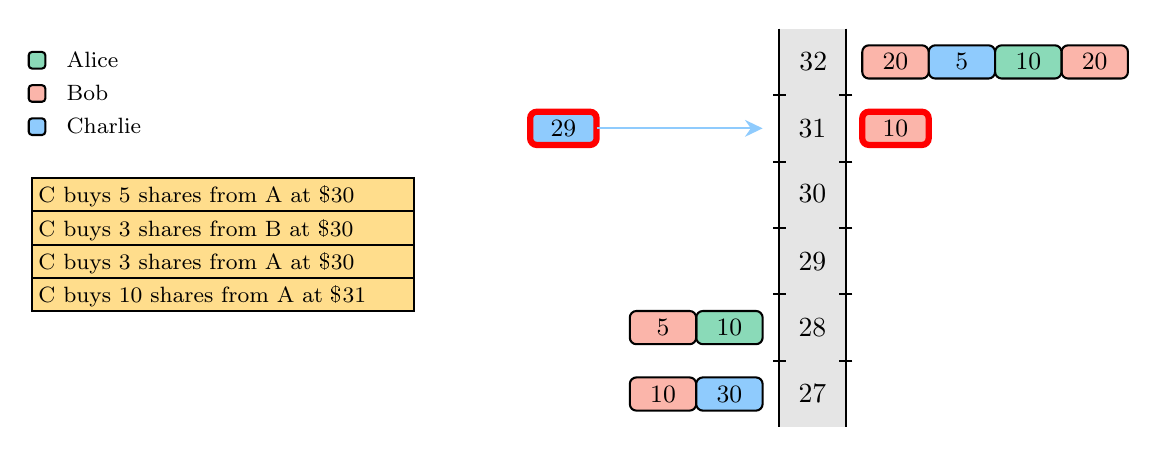
\begin{tikzpicture}[x=0.75pt,y=0.75pt,yscale=-0.8,xscale=0.8]
%uncomment if require: \path (0,300); %set diagram left start at 0, and has height of 300


%Shape: Rectangle [id:dp8337814582471778] 
\draw  [draw opacity=0][fill={rgb, 255:red, 0; green, 0; blue, 0 }  ,fill opacity=0.1 ] (470,40) -- (510,40) -- (510,280) -- (470,280) -- cycle ;
%Straight Lines [id:da09969873094924853] 
\draw    (470,40) -- (470,280) (474,80) -- (466,80)(474,120) -- (466,120)(474,160) -- (466,160)(474,200) -- (466,200)(474,240) -- (466,240) ;
%Straight Lines [id:da5936664441336669] 
\draw    (510,40) -- (510,280) (514,80) -- (506,80)(514,120) -- (506,120)(514,160) -- (506,160)(514,200) -- (506,200)(514,240) -- (506,240) ;
%Rounded Rect [id:dp21774022020109518] 
\draw  [fill={rgb, 255:red, 138; green, 218; blue, 184 }  ,fill opacity=1 ][line width=0.75]  (420,214) .. controls (420,211.79) and (421.79,210) .. (424,210) -- (456,210) .. controls (458.21,210) and (460,211.79) .. (460,214) -- (460,226) .. controls (460,228.21) and (458.21,230) .. (456,230) -- (424,230) .. controls (421.79,230) and (420,228.21) .. (420,226) -- cycle ;
%Rounded Rect [id:dp27872897957842435] 
\draw  [fill={rgb, 255:red, 251; green, 181; blue, 170 }  ,fill opacity=1 ][line width=0.75]  (380,214) .. controls (380,211.79) and (381.79,210) .. (384,210) -- (416,210) .. controls (418.21,210) and (420,211.79) .. (420,214) -- (420,226) .. controls (420,228.21) and (418.21,230) .. (416,230) -- (384,230) .. controls (381.79,230) and (380,228.21) .. (380,226) -- cycle ;
%Rounded Rect [id:dp2087008923376935] 
\draw  [fill={rgb, 255:red, 251; green, 181; blue, 170 }  ,fill opacity=1 ][line width=0.75]  (380,254) .. controls (380,251.79) and (381.79,250) .. (384,250) -- (416,250) .. controls (418.21,250) and (420,251.79) .. (420,254) -- (420,266) .. controls (420,268.21) and (418.21,270) .. (416,270) -- (384,270) .. controls (381.79,270) and (380,268.21) .. (380,266) -- cycle ;
%Rounded Rect [id:dp1281757847349283] 
\draw  [fill={rgb, 255:red, 138; green, 218; blue, 184 }  ,fill opacity=1 ][line width=0.75]  (18,56) .. controls (18,54.9) and (18.9,54) .. (20,54) -- (26,54) .. controls (27.1,54) and (28,54.9) .. (28,56) -- (28,62) .. controls (28,63.1) and (27.1,64) .. (26,64) -- (20,64) .. controls (18.9,64) and (18,63.1) .. (18,62) -- cycle ;
%Rounded Rect [id:dp9520385717692255] 
\draw  [fill={rgb, 255:red, 143; green, 203; blue, 253 }  ,fill opacity=1 ][line width=0.75]  (18,96) .. controls (18,94.9) and (18.9,94) .. (20,94) -- (26,94) .. controls (27.1,94) and (28,94.9) .. (28,96) -- (28,102) .. controls (28,103.1) and (27.1,104) .. (26,104) -- (20,104) .. controls (18.9,104) and (18,103.1) .. (18,102) -- cycle ;
%Rounded Rect [id:dp4915947371569024] 
\draw  [fill={rgb, 255:red, 251; green, 181; blue, 170 }  ,fill opacity=1 ][line width=0.75]  (18,76) .. controls (18,74.9) and (18.9,74) .. (20,74) -- (26,74) .. controls (27.1,74) and (28,74.9) .. (28,76) -- (28,82) .. controls (28,83.1) and (27.1,84) .. (26,84) -- (20,84) .. controls (18.9,84) and (18,83.1) .. (18,82) -- cycle ;
%Rounded Rect [id:dp1657885524180357] 
\draw  [color={rgb, 255:red, 255; green, 0; blue, 0 }  ,draw opacity=1 ][fill={rgb, 255:red, 251; green, 181; blue, 170 }  ,fill opacity=1 ][line width=2.25]  (520,94) .. controls (520,91.79) and (521.79,90) .. (524,90) -- (556,90) .. controls (558.21,90) and (560,91.79) .. (560,94) -- (560,106) .. controls (560,108.21) and (558.21,110) .. (556,110) -- (524,110) .. controls (521.79,110) and (520,108.21) .. (520,106) -- cycle ;
%Rounded Rect [id:dp19440278883646667] 
\draw  [fill={rgb, 255:red, 143; green, 203; blue, 253 }  ,fill opacity=1 ][line width=0.75]  (560,54) .. controls (560,51.79) and (561.79,50) .. (564,50) -- (596,50) .. controls (598.21,50) and (600,51.79) .. (600,54) -- (600,66) .. controls (600,68.21) and (598.21,70) .. (596,70) -- (564,70) .. controls (561.79,70) and (560,68.21) .. (560,66) -- cycle ;
%Rounded Rect [id:dp11444604878691622] 
\draw  [fill={rgb, 255:red, 143; green, 203; blue, 253 }  ,fill opacity=1 ][line width=0.75]  (420,254) .. controls (420,251.79) and (421.79,250) .. (424,250) -- (456,250) .. controls (458.21,250) and (460,251.79) .. (460,254) -- (460,266) .. controls (460,268.21) and (458.21,270) .. (456,270) -- (424,270) .. controls (421.79,270) and (420,268.21) .. (420,266) -- cycle ;
%Rounded Rect [id:dp6379504097709302] 
\draw  [color={rgb, 255:red, 255; green, 0; blue, 0 }  ,draw opacity=1 ][fill={rgb, 255:red, 143; green, 203; blue, 253 }  ,fill opacity=1 ][line width=2.25]  (320,94) .. controls (320,91.79) and (321.79,90) .. (324,90) -- (356,90) .. controls (358.21,90) and (360,91.79) .. (360,94) -- (360,106) .. controls (360,108.21) and (358.21,110) .. (356,110) -- (324,110) .. controls (321.79,110) and (320,108.21) .. (320,106) -- cycle ;
%Straight Lines [id:da5639250481518682] 
\draw [color={rgb, 255:red, 143; green, 203; blue, 253 }  ,draw opacity=1 ]   (360,100) -- (457,100) ;
\draw [shift={(460,100)}, rotate = 180] [fill={rgb, 255:red, 143; green, 203; blue, 253 }  ,fill opacity=1 ][line width=0.08]  [draw opacity=0] (10.72,-5.15) -- (0,0) -- (10.72,5.15) -- (7.12,0) -- cycle    ;
%Rounded Rect [id:dp7706984934543188] 
\draw  [fill={rgb, 255:red, 251; green, 181; blue, 170 }  ,fill opacity=1 ][line width=0.75]  (520,54) .. controls (520,51.79) and (521.79,50) .. (524,50) -- (556,50) .. controls (558.21,50) and (560,51.79) .. (560,54) -- (560,66) .. controls (560,68.21) and (558.21,70) .. (556,70) -- (524,70) .. controls (521.79,70) and (520,68.21) .. (520,66) -- cycle ;
%Rounded Rect [id:dp49004438558198016] 
\draw  [fill={rgb, 255:red, 251; green, 181; blue, 170 }  ,fill opacity=1 ][line width=0.75]  (640,54) .. controls (640,51.79) and (641.79,50) .. (644,50) -- (676,50) .. controls (678.21,50) and (680,51.79) .. (680,54) -- (680,66) .. controls (680,68.21) and (678.21,70) .. (676,70) -- (644,70) .. controls (641.79,70) and (640,68.21) .. (640,66) -- cycle ;
%Rounded Rect [id:dp17939821006978351] 
\draw  [fill={rgb, 255:red, 138; green, 218; blue, 184 }  ,fill opacity=1 ][line width=0.75]  (600,54) .. controls (600,51.79) and (601.79,50) .. (604,50) -- (636,50) .. controls (638.21,50) and (640,51.79) .. (640,54) -- (640,66) .. controls (640,68.21) and (638.21,70) .. (636,70) -- (604,70) .. controls (601.79,70) and (600,68.21) .. (600,66) -- cycle ;
%Shape: Rectangle [id:dp9403473417630838] 
\draw  [fill={rgb, 255:red, 255; green, 221; blue, 140 }  ,fill opacity=1 ] (20,130) -- (250,130) -- (250,150) -- (20,150) -- cycle ;
%Shape: Rectangle [id:dp49072857961828886] 
\draw  [fill={rgb, 255:red, 255; green, 221; blue, 140 }  ,fill opacity=1 ] (20,150) -- (250,150) -- (250,170) -- (20,170) -- cycle ;
%Shape: Rectangle [id:dp9961567428739467] 
\draw  [fill={rgb, 255:red, 255; green, 221; blue, 140 }  ,fill opacity=1 ] (20,190) -- (250,190) -- (250,210) -- (20,210) -- cycle ;
%Shape: Rectangle [id:dp3060916994428581] 
\draw  [fill={rgb, 255:red, 255; green, 221; blue, 140 }  ,fill opacity=1 ] (20,170) -- (250,170) -- (250,190) -- (20,190) -- cycle ;

% Text Node
\draw (490,100) node    {$31$};
% Text Node
\draw (490,139.5) node    {$30$};
% Text Node
\draw (490,180) node    {$29$};
% Text Node
\draw (490,220) node    {$28$};
% Text Node
\draw (490,260) node    {$27$};
% Text Node
\draw (440,220) node  [font=\small]  {$10$};
% Text Node
\draw (400,220) node  [font=\small]  {${\textstyle 5}$};
% Text Node
\draw (400,260) node  [font=\small]  {$10$};
% Text Node
\draw (39,52) node [anchor=north west][inner sep=0.75pt]  [font=\footnotesize] [align=left] {Alice};
% Text Node
\draw (39,72) node [anchor=north west][inner sep=0.75pt]  [font=\footnotesize] [align=left] {Bob};
% Text Node
\draw (39,92) node [anchor=north west][inner sep=0.75pt]  [font=\footnotesize] [align=left] {Charlie};
% Text Node
\draw (540,100) node  [font=\small]  {$10$};
% Text Node
\draw (490.5,60) node    {$32$};
% Text Node
\draw (580,60) node  [font=\small]  {$5$};
% Text Node
\draw (440,260) node  [font=\small]  {$30$};
% Text Node
\draw (340,100) node  [font=\small]  {$29$};
% Text Node
\draw (540,60) node  [font=\small]  {$20$};
% Text Node
\draw (660,60) node  [font=\small]  {$20$};
% Text Node
\draw (620,60) node  [font=\small]  {$10$};
% Text Node
\draw (22,133) node [anchor=north west][inner sep=0.75pt] [font=\footnotesize] [align=left] {C buys 5 shares from A at \$30};
% Text Node
\draw (22,153) node [anchor=north west][inner sep=0.75pt] [font=\footnotesize] [align=left] {C buys 3 shares from B at \$30};
% Text Node
\draw (22,193) node [anchor=north west][inner sep=0.75pt] [font=\footnotesize] [align=left] {C buys 10 shares from A at \$31};
% Text Node
\draw (22,173) node [anchor=north west][inner sep=0.75pt] [font=\footnotesize] [align=left] {C buys 3 shares from A at \$30};


\end{tikzpicture}
}
    \only<6>{

\tikzset{every picture/.style={line width=0.75pt}} %set default line width to 0.75pt        

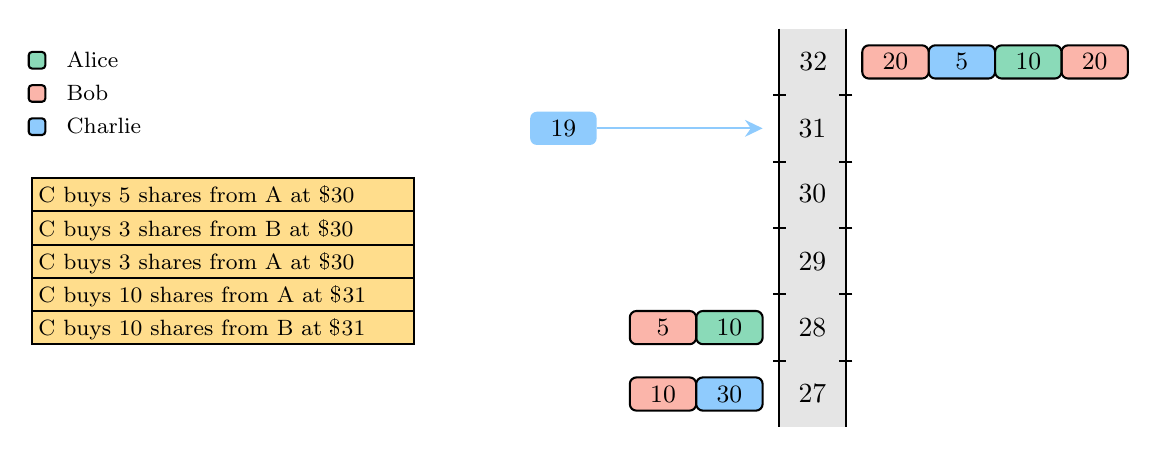
\begin{tikzpicture}[x=0.75pt,y=0.75pt,yscale=-0.8,xscale=0.8]
%uncomment if require: \path (0,300); %set diagram left start at 0, and has height of 300

%Shape: Rectangle [id:dp3861715993266832] 
\draw  [draw opacity=0][fill={rgb, 255:red, 0; green, 0; blue, 0 }  ,fill opacity=0.1 ] (470,40) -- (510,40) -- (510,280) -- (470,280) -- cycle ;
%Straight Lines [id:da8309385407681799] 
\draw    (470,40) -- (470,280) (474,80) -- (466,80)(474,120) -- (466,120)(474,160) -- (466,160)(474,200) -- (466,200)(474,240) -- (466,240) ;
%Straight Lines [id:da5801335245942738] 
\draw    (510,40) -- (510,280) (514,80) -- (506,80)(514,120) -- (506,120)(514,160) -- (506,160)(514,200) -- (506,200)(514,240) -- (506,240) ;
%Rounded Rect [id:dp937444837474773] 
\draw  [fill={rgb, 255:red, 138; green, 218; blue, 184 }  ,fill opacity=1 ][line width=0.75]  (420,214) .. controls (420,211.79) and (421.79,210) .. (424,210) -- (456,210) .. controls (458.21,210) and (460,211.79) .. (460,214) -- (460,226) .. controls (460,228.21) and (458.21,230) .. (456,230) -- (424,230) .. controls (421.79,230) and (420,228.21) .. (420,226) -- cycle ;
%Rounded Rect [id:dp6370281869352094] 
\draw  [fill={rgb, 255:red, 251; green, 181; blue, 170 }  ,fill opacity=1 ][line width=0.75]  (380,214) .. controls (380,211.79) and (381.79,210) .. (384,210) -- (416,210) .. controls (418.21,210) and (420,211.79) .. (420,214) -- (420,226) .. controls (420,228.21) and (418.21,230) .. (416,230) -- (384,230) .. controls (381.79,230) and (380,228.21) .. (380,226) -- cycle ;
%Rounded Rect [id:dp9214685747053574] 
\draw  [fill={rgb, 255:red, 251; green, 181; blue, 170 }  ,fill opacity=1 ][line width=0.75]  (380,254) .. controls (380,251.79) and (381.79,250) .. (384,250) -- (416,250) .. controls (418.21,250) and (420,251.79) .. (420,254) -- (420,266) .. controls (420,268.21) and (418.21,270) .. (416,270) -- (384,270) .. controls (381.79,270) and (380,268.21) .. (380,266) -- cycle ;
%Rounded Rect [id:dp5437621877409694] 
\draw  [fill={rgb, 255:red, 138; green, 218; blue, 184 }  ,fill opacity=1 ][line width=0.75]  (18,56) .. controls (18,54.9) and (18.9,54) .. (20,54) -- (26,54) .. controls (27.1,54) and (28,54.9) .. (28,56) -- (28,62) .. controls (28,63.1) and (27.1,64) .. (26,64) -- (20,64) .. controls (18.9,64) and (18,63.1) .. (18,62) -- cycle ;
%Rounded Rect [id:dp09068402110649876] 
\draw  [fill={rgb, 255:red, 143; green, 203; blue, 253 }  ,fill opacity=1 ][line width=0.75]  (18,96) .. controls (18,94.9) and (18.9,94) .. (20,94) -- (26,94) .. controls (27.1,94) and (28,94.9) .. (28,96) -- (28,102) .. controls (28,103.1) and (27.1,104) .. (26,104) -- (20,104) .. controls (18.9,104) and (18,103.1) .. (18,102) -- cycle ;
%Rounded Rect [id:dp6353505724561966] 
\draw  [fill={rgb, 255:red, 251; green, 181; blue, 170 }  ,fill opacity=1 ][line width=0.75]  (18,76) .. controls (18,74.9) and (18.9,74) .. (20,74) -- (26,74) .. controls (27.1,74) and (28,74.9) .. (28,76) -- (28,82) .. controls (28,83.1) and (27.1,84) .. (26,84) -- (20,84) .. controls (18.9,84) and (18,83.1) .. (18,82) -- cycle ;
%Rounded Rect [id:dp6699541273577541] 
\draw  [fill={rgb, 255:red, 143; green, 203; blue, 253 }  ,fill opacity=1 ][line width=0.75]  (560,54) .. controls (560,51.79) and (561.79,50) .. (564,50) -- (596,50) .. controls (598.21,50) and (600,51.79) .. (600,54) -- (600,66) .. controls (600,68.21) and (598.21,70) .. (596,70) -- (564,70) .. controls (561.79,70) and (560,68.21) .. (560,66) -- cycle ;
%Rounded Rect [id:dp9726118728538371] 
\draw  [fill={rgb, 255:red, 143; green, 203; blue, 253 }  ,fill opacity=1 ][line width=0.75]  (420,254) .. controls (420,251.79) and (421.79,250) .. (424,250) -- (456,250) .. controls (458.21,250) and (460,251.79) .. (460,254) -- (460,266) .. controls (460,268.21) and (458.21,270) .. (456,270) -- (424,270) .. controls (421.79,270) and (420,268.21) .. (420,266) -- cycle ;
%Rounded Rect [id:dp36723448056690344] 
\draw  [draw opacity=0][fill={rgb, 255:red, 143; green, 203; blue, 253 }  ,fill opacity=1 ][line width=2.25]  (320,94) .. controls (320,91.79) and (321.79,90) .. (324,90) -- (356,90) .. controls (358.21,90) and (360,91.79) .. (360,94) -- (360,106) .. controls (360,108.21) and (358.21,110) .. (356,110) -- (324,110) .. controls (321.79,110) and (320,108.21) .. (320,106) -- cycle ;
%Straight Lines [id:da6684571902186517] 
\draw [color={rgb, 255:red, 143; green, 203; blue, 253 }  ,draw opacity=1 ]   (360,100) -- (457,100) ;
\draw [shift={(460,100)}, rotate = 180] [fill={rgb, 255:red, 143; green, 203; blue, 253 }  ,fill opacity=1 ][line width=0.08]  [draw opacity=0] (10.72,-5.15) -- (0,0) -- (10.72,5.15) -- (7.12,0) -- cycle    ;
%Rounded Rect [id:dp38795887413284924] 
\draw  [fill={rgb, 255:red, 251; green, 181; blue, 170 }  ,fill opacity=1 ][line width=0.75]  (520,54) .. controls (520,51.79) and (521.79,50) .. (524,50) -- (556,50) .. controls (558.21,50) and (560,51.79) .. (560,54) -- (560,66) .. controls (560,68.21) and (558.21,70) .. (556,70) -- (524,70) .. controls (521.79,70) and (520,68.21) .. (520,66) -- cycle ;
%Rounded Rect [id:dp9194433328726554] 
\draw  [fill={rgb, 255:red, 251; green, 181; blue, 170 }  ,fill opacity=1 ][line width=0.75]  (640,54) .. controls (640,51.79) and (641.79,50) .. (644,50) -- (676,50) .. controls (678.21,50) and (680,51.79) .. (680,54) -- (680,66) .. controls (680,68.21) and (678.21,70) .. (676,70) -- (644,70) .. controls (641.79,70) and (640,68.21) .. (640,66) -- cycle ;
%Rounded Rect [id:dp3212198976203209] 
\draw  [fill={rgb, 255:red, 138; green, 218; blue, 184 }  ,fill opacity=1 ][line width=0.75]  (600,54) .. controls (600,51.79) and (601.79,50) .. (604,50) -- (636,50) .. controls (638.21,50) and (640,51.79) .. (640,54) -- (640,66) .. controls (640,68.21) and (638.21,70) .. (636,70) -- (604,70) .. controls (601.79,70) and (600,68.21) .. (600,66) -- cycle ;
%Shape: Rectangle [id:dp08517938360246491] 
\draw  [fill={rgb, 255:red, 255; green, 221; blue, 140 }  ,fill opacity=1 ] (20,130) -- (250,130) -- (250,150) -- (20,150) -- cycle ;
%Shape: Rectangle [id:dp06032042157532158] 
\draw  [fill={rgb, 255:red, 255; green, 221; blue, 140 }  ,fill opacity=1 ] (20,150) -- (250,150) -- (250,170) -- (20,170) -- cycle ;
%Shape: Rectangle [id:dp4098790697085256] 
\draw  [fill={rgb, 255:red, 255; green, 221; blue, 140 }  ,fill opacity=1 ] (20,190) -- (250,190) -- (250,210) -- (20,210) -- cycle ;
%Shape: Rectangle [id:dp1707508013100606] 
\draw  [fill={rgb, 255:red, 255; green, 221; blue, 140 }  ,fill opacity=1 ] (20,170) -- (250,170) -- (250,190) -- (20,190) -- cycle ;
%Shape: Rectangle [id:dp9028347275422166] 
\draw  [fill={rgb, 255:red, 255; green, 221; blue, 140 }  ,fill opacity=1 ] (20,210) -- (250,210) -- (250,230) -- (20,230) -- cycle ;

% Text Node
\draw (490,100) node    {$31$};
% Text Node
\draw (490,139.5) node    {$30$};
% Text Node
\draw (490,180) node    {$29$};
% Text Node
\draw (490,220) node    {$28$};
% Text Node
\draw (490,260) node    {$27$};
% Text Node
\draw (440,220) node  [font=\small]  {$10$};
% Text Node
\draw (400,220) node  [font=\small]  {${\textstyle 5}$};
% Text Node
\draw (400,260) node  [font=\small]  {$10$};
% Text Node
\draw (39,52) node [anchor=north west][inner sep=0.75pt]  [font=\footnotesize] [align=left] {Alice};
% Text Node
\draw (39,72) node [anchor=north west][inner sep=0.75pt]  [font=\footnotesize] [align=left] {Bob};
% Text Node
\draw (39,92) node [anchor=north west][inner sep=0.75pt]  [font=\footnotesize] [align=left] {Charlie};
% Text Node
\draw (490.5,60) node    {$32$};
% Text Node
\draw (580,60) node  [font=\small]  {$5$};
% Text Node
\draw (440,260) node  [font=\small]  {$30$};
% Text Node
\draw (340,100) node  [font=\small]  {$19$};
% Text Node
\draw (540,60) node  [font=\small]  {$20$};
% Text Node
\draw (660,60) node  [font=\small]  {$20$};
% Text Node
\draw (620,60) node  [font=\small]  {$10$};
% Text Node
\draw (22,133) node [anchor=north west][inner sep=0.75pt] [font=\footnotesize] [align=left] {C buys 5 shares from A at \$30};
% Text Node
\draw (22,153) node [anchor=north west][inner sep=0.75pt] [font=\footnotesize] [align=left] {C buys 3 shares from B at \$30};
% Text Node
\draw (22,193) node [anchor=north west][inner sep=0.75pt] [font=\footnotesize] [align=left] {C buys 10 shares from A at \$31};
% Text Node
\draw (22,173) node [anchor=north west][inner sep=0.75pt] [font=\footnotesize] [align=left] {C buys 3 shares from A at \$30};
% Text Node
\draw (22,213) node [anchor=north west][inner sep=0.75pt] [font=\footnotesize] [align=left] {C buys 10 shares from B at \$31};


\end{tikzpicture}
}
  \end{center}
\end{frame}

\begin{frame}{Large GTC Buy Order: Result}
  \begin{center}
    \input{assets/large_gtc_frame_result.tex}
  \end{center}
\end{frame}

\begin{frame}{Aggregated Orderbook}
  \begin{sqt:result}
    Usually, exchanges only reveal to the participants:
    \begin{itemize}
      \item the set of \textbf{their own} open orders
      \item the \textbf{aggregated} orderbook (all quantities on each level are aggregated)
    \end{itemize}
  \end{sqt:result}

  \begin{center}
    

\tikzset{every picture/.style={line width=0.75pt}} %set default line width to 0.75pt        

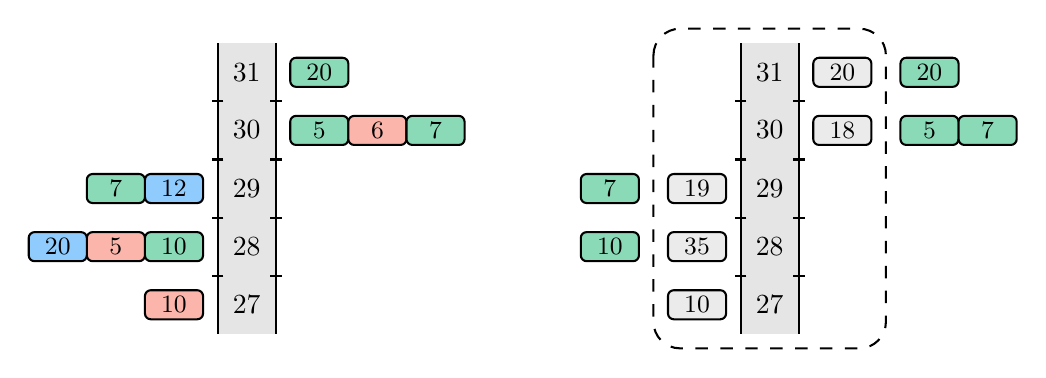
\begin{tikzpicture}[x=0.75pt,y=0.75pt,yscale=-0.7,xscale=0.7]
%uncomment if require: \path (0,300); %set diagram left start at 0, and has height of 300


%Shape: Rectangle [id:dp5489135505501248] 
\draw  [draw opacity=0][fill={rgb, 255:red, 0; green, 0; blue, 0 }  ,fill opacity=0.1 ] (140,60) -- (180,60) -- (180,260) -- (140,260) -- cycle ;
%Rounded Rect [id:dp5571720629473116] 
\draw  [fill={rgb, 255:red, 138; green, 218; blue, 184 }  ,fill opacity=1 ][line width=0.75]  (190,114) .. controls (190,111.79) and (191.79,110) .. (194,110) -- (226,110) .. controls (228.21,110) and (230,111.79) .. (230,114) -- (230,126) .. controls (230,128.21) and (228.21,130) .. (226,130) -- (194,130) .. controls (191.79,130) and (190,128.21) .. (190,126) -- cycle ;
%Straight Lines [id:da6082688802942293] 
\draw    (140,60) -- (140,260) (144,100) -- (136,100)(144,140) -- (136,140)(144,180) -- (136,180)(144,220) -- (136,220) ;
%Straight Lines [id:da9720053745263018] 
\draw    (180,60) -- (180,260) (184,100) -- (176,100)(184,140) -- (176,140)(184,180) -- (176,180)(184,220) -- (176,220) ;
%Rounded Rect [id:dp10362529279551769] 
\draw  [fill={rgb, 255:red, 251; green, 181; blue, 170 }  ,fill opacity=1 ][line width=0.75]  (230,114) .. controls (230,111.79) and (231.79,110) .. (234,110) -- (266,110) .. controls (268.21,110) and (270,111.79) .. (270,114) -- (270,126) .. controls (270,128.21) and (268.21,130) .. (266,130) -- (234,130) .. controls (231.79,130) and (230,128.21) .. (230,126) -- cycle ;
%Rounded Rect [id:dp3209795107013548] 
\draw  [fill={rgb, 255:red, 138; green, 218; blue, 184 }  ,fill opacity=1 ][line width=0.75]  (270,114) .. controls (270,111.79) and (271.79,110) .. (274,110) -- (306,110) .. controls (308.21,110) and (310,111.79) .. (310,114) -- (310,126) .. controls (310,128.21) and (308.21,130) .. (306,130) -- (274,130) .. controls (271.79,130) and (270,128.21) .. (270,126) -- cycle ;
%Rounded Rect [id:dp14006433626528436] 
\draw  [fill={rgb, 255:red, 138; green, 218; blue, 184 }  ,fill opacity=1 ][line width=0.75]  (190,74) .. controls (190,71.79) and (191.79,70) .. (194,70) -- (226,70) .. controls (228.21,70) and (230,71.79) .. (230,74) -- (230,86) .. controls (230,88.21) and (228.21,90) .. (226,90) -- (194,90) .. controls (191.79,90) and (190,88.21) .. (190,86) -- cycle ;
%Rounded Rect [id:dp23032489064391803] 
\draw  [fill={rgb, 255:red, 138; green, 218; blue, 184 }  ,fill opacity=1 ][line width=0.75]  (90,194) .. controls (90,191.79) and (91.79,190) .. (94,190) -- (126,190) .. controls (128.21,190) and (130,191.79) .. (130,194) -- (130,206) .. controls (130,208.21) and (128.21,210) .. (126,210) -- (94,210) .. controls (91.79,210) and (90,208.21) .. (90,206) -- cycle ;
%Rounded Rect [id:dp2906178876656058] 
\draw  [fill={rgb, 255:red, 143; green, 203; blue, 253 }  ,fill opacity=1 ][line width=0.75]  (90,154) .. controls (90,151.79) and (91.79,150) .. (94,150) -- (126,150) .. controls (128.21,150) and (130,151.79) .. (130,154) -- (130,166) .. controls (130,168.21) and (128.21,170) .. (126,170) -- (94,170) .. controls (91.79,170) and (90,168.21) .. (90,166) -- cycle ;
%Rounded Rect [id:dp2773205270553206] 
\draw  [fill={rgb, 255:red, 138; green, 218; blue, 184 }  ,fill opacity=1 ][line width=0.75]  (50,154) .. controls (50,151.79) and (51.79,150) .. (54,150) -- (86,150) .. controls (88.21,150) and (90,151.79) .. (90,154) -- (90,166) .. controls (90,168.21) and (88.21,170) .. (86,170) -- (54,170) .. controls (51.79,170) and (50,168.21) .. (50,166) -- cycle ;
%Rounded Rect [id:dp4559050638577514] 
\draw  [fill={rgb, 255:red, 251; green, 181; blue, 170 }  ,fill opacity=1 ][line width=0.75]  (50,194) .. controls (50,191.79) and (51.79,190) .. (54,190) -- (86,190) .. controls (88.21,190) and (90,191.79) .. (90,194) -- (90,206) .. controls (90,208.21) and (88.21,210) .. (86,210) -- (54,210) .. controls (51.79,210) and (50,208.21) .. (50,206) -- cycle ;
%Rounded Rect [id:dp12376095296435441] 
\draw  [fill={rgb, 255:red, 143; green, 203; blue, 253 }  ,fill opacity=1 ][line width=0.75]  (10,194) .. controls (10,191.79) and (11.79,190) .. (14,190) -- (46,190) .. controls (48.21,190) and (50,191.79) .. (50,194) -- (50,206) .. controls (50,208.21) and (48.21,210) .. (46,210) -- (14,210) .. controls (11.79,210) and (10,208.21) .. (10,206) -- cycle ;
%Rounded Rect [id:dp5644180007175256] 
\draw  [fill={rgb, 255:red, 251; green, 181; blue, 170 }  ,fill opacity=1 ][line width=0.75]  (90,234) .. controls (90,231.79) and (91.79,230) .. (94,230) -- (126,230) .. controls (128.21,230) and (130,231.79) .. (130,234) -- (130,246) .. controls (130,248.21) and (128.21,250) .. (126,250) -- (94,250) .. controls (91.79,250) and (90,248.21) .. (90,246) -- cycle ;
%Shape: Rectangle [id:dp5662774353889877] 
\draw  [draw opacity=0][fill={rgb, 255:red, 0; green, 0; blue, 0 }  ,fill opacity=0.1 ] (500,60) -- (540,60) -- (540,260) -- (500,260) -- cycle ;
%Rounded Rect [id:dp08118930746789832] 
\draw  [fill={rgb, 255:red, 235; green, 235; blue, 235 }  ,fill opacity=1 ][line width=0.75]  (550,114) .. controls (550,111.79) and (551.79,110) .. (554,110) -- (586,110) .. controls (588.21,110) and (590,111.79) .. (590,114) -- (590,126) .. controls (590,128.21) and (588.21,130) .. (586,130) -- (554,130) .. controls (551.79,130) and (550,128.21) .. (550,126) -- cycle ;
%Straight Lines [id:da20677085553463082] 
\draw    (500,60) -- (500,260) (504,100) -- (496,100)(504,140) -- (496,140)(504,180) -- (496,180)(504,220) -- (496,220) ;
%Straight Lines [id:da40710486463167805] 
\draw    (540,60) -- (540,260) (544,100) -- (536,100)(544,140) -- (536,140)(544,180) -- (536,180)(544,220) -- (536,220) ;
%Rounded Rect [id:dp6364145985594639] 
\draw  [fill={rgb, 255:red, 235; green, 235; blue, 235 }  ,fill opacity=1 ][line width=0.75]  (550,74) .. controls (550,71.79) and (551.79,70) .. (554,70) -- (586,70) .. controls (588.21,70) and (590,71.79) .. (590,74) -- (590,86) .. controls (590,88.21) and (588.21,90) .. (586,90) -- (554,90) .. controls (551.79,90) and (550,88.21) .. (550,86) -- cycle ;
%Rounded Rect [id:dp2804611471386602] 
\draw  [fill={rgb, 255:red, 235; green, 235; blue, 235 }  ,fill opacity=1 ][line width=0.75]  (450,194) .. controls (450,191.79) and (451.79,190) .. (454,190) -- (486,190) .. controls (488.21,190) and (490,191.79) .. (490,194) -- (490,206) .. controls (490,208.21) and (488.21,210) .. (486,210) -- (454,210) .. controls (451.79,210) and (450,208.21) .. (450,206) -- cycle ;
%Rounded Rect [id:dp24217444343409034] 
\draw  [fill={rgb, 255:red, 235; green, 235; blue, 235 }  ,fill opacity=1 ][line width=0.75]  (450,154) .. controls (450,151.79) and (451.79,150) .. (454,150) -- (486,150) .. controls (488.21,150) and (490,151.79) .. (490,154) -- (490,166) .. controls (490,168.21) and (488.21,170) .. (486,170) -- (454,170) .. controls (451.79,170) and (450,168.21) .. (450,166) -- cycle ;
%Rounded Rect [id:dp045526064729431215] 
\draw  [fill={rgb, 255:red, 235; green, 235; blue, 235 }  ,fill opacity=1 ][line width=0.75]  (450,234) .. controls (450,231.79) and (451.79,230) .. (454,230) -- (486,230) .. controls (488.21,230) and (490,231.79) .. (490,234) -- (490,246) .. controls (490,248.21) and (488.21,250) .. (486,250) -- (454,250) .. controls (451.79,250) and (450,248.21) .. (450,246) -- cycle ;
%Rounded Rect [id:dp6633295562595507] 
\draw  [fill={rgb, 255:red, 138; green, 218; blue, 184 }  ,fill opacity=1 ][line width=0.75]  (390,194) .. controls (390,191.79) and (391.79,190) .. (394,190) -- (426,190) .. controls (428.21,190) and (430,191.79) .. (430,194) -- (430,206) .. controls (430,208.21) and (428.21,210) .. (426,210) -- (394,210) .. controls (391.79,210) and (390,208.21) .. (390,206) -- cycle ;
%Rounded Rect [id:dp641336334884714] 
\draw  [fill={rgb, 255:red, 138; green, 218; blue, 184 }  ,fill opacity=1 ][line width=0.75]  (390,154) .. controls (390,151.79) and (391.79,150) .. (394,150) -- (426,150) .. controls (428.21,150) and (430,151.79) .. (430,154) -- (430,166) .. controls (430,168.21) and (428.21,170) .. (426,170) -- (394,170) .. controls (391.79,170) and (390,168.21) .. (390,166) -- cycle ;
%Rounded Rect [id:dp4238339096677155] 
\draw  [fill={rgb, 255:red, 138; green, 218; blue, 184 }  ,fill opacity=1 ][line width=0.75]  (610,114) .. controls (610,111.79) and (611.79,110) .. (614,110) -- (646,110) .. controls (648.21,110) and (650,111.79) .. (650,114) -- (650,126) .. controls (650,128.21) and (648.21,130) .. (646,130) -- (614,130) .. controls (611.79,130) and (610,128.21) .. (610,126) -- cycle ;
%Rounded Rect [id:dp3352222243665929] 
\draw  [fill={rgb, 255:red, 138; green, 218; blue, 184 }  ,fill opacity=1 ][line width=0.75]  (650,114) .. controls (650,111.79) and (651.79,110) .. (654,110) -- (686,110) .. controls (688.21,110) and (690,111.79) .. (690,114) -- (690,126) .. controls (690,128.21) and (688.21,130) .. (686,130) -- (654,130) .. controls (651.79,130) and (650,128.21) .. (650,126) -- cycle ;
%Rounded Rect [id:dp018044766031021897] 
\draw  [fill={rgb, 255:red, 138; green, 218; blue, 184 }  ,fill opacity=1 ][line width=0.75]  (610,74) .. controls (610,71.79) and (611.79,70) .. (614,70) -- (646,70) .. controls (648.21,70) and (650,71.79) .. (650,74) -- (650,86) .. controls (650,88.21) and (648.21,90) .. (646,90) -- (614,90) .. controls (611.79,90) and (610,88.21) .. (610,86) -- cycle ;
%Rounded Rect [id:dp43481833872293096] 
\draw  [dash pattern={on 4.5pt off 4.5pt}] (440,68.3) .. controls (440,58.19) and (448.19,50) .. (458.3,50) -- (581.7,50) .. controls (591.81,50) and (600,58.19) .. (600,68.3) -- (600,251.7) .. controls (600,261.81) and (591.81,270) .. (581.7,270) -- (458.3,270) .. controls (448.19,270) and (440,261.81) .. (440,251.7) -- cycle ;

% Text Node
\draw (160,80) node    {$31$};
% Text Node
\draw (160,119.5) node    {$30$};
% Text Node
\draw (210,120) node  [font=\small]  {${\textstyle 5}$};
% Text Node
\draw (160,160) node    {$29$};
% Text Node
\draw (160,200) node    {$28$};
% Text Node
\draw (160,240) node    {$27$};
% Text Node
\draw (250,120) node  [font=\small]  {$6$};
% Text Node
\draw (290,120) node  [font=\small]  {$7$};
% Text Node
\draw (210,80) node  [font=\small]  {$20$};
% Text Node
\draw (110,200) node  [font=\small]  {$10$};
% Text Node
\draw (110,160) node  [font=\small]  {$12$};
% Text Node
\draw (70,160) node  [font=\small]  {$7$};
% Text Node
\draw (70,200) node  [font=\small]  {${\textstyle 5}$};
% Text Node
\draw (30,200) node  [font=\small]  {$20$};
% Text Node
\draw (110,240) node  [font=\small]  {$10$};
% Text Node
\draw (520,80) node    {$31$};
% Text Node
\draw (520,119.5) node    {$30$};
% Text Node
\draw (570,120) node  [font=\small]  {$18$};
% Text Node
\draw (520,160) node    {$29$};
% Text Node
\draw (520,200) node    {$28$};
% Text Node
\draw (520,240) node    {$27$};
% Text Node
\draw (570,80) node  [font=\small]  {$20$};
% Text Node
\draw (470,200) node  [font=\small]  {$35$};
% Text Node
\draw (470,160) node  [font=\small]  {$19$};
% Text Node
\draw (470,240) node  [font=\small]  {$10$};
% Text Node
\draw (410,200) node  [font=\small]  {$10$};
% Text Node
\draw (410,160) node  [font=\small]  {$7$};
% Text Node
\draw (630,120) node  [font=\small]  {$5$};
% Text Node
\draw (670,120) node  [font=\small]  {$7$};
% Text Node
\draw (630,80) node  [font=\small]  {$20$};


\end{tikzpicture}

  \end{center}
\end{frame}

\begin{frame}{Liquidity and Market Impact}
  \begin{sqt:definition}
    An orderbook with tight spreads and large volume is considered \textbf{liquid}.
  \end{sqt:definition}

  In an \textbf{illiquid} market, orders can \textbf{eat through} the orderbook.\\
  \textbf{Market impact} is when an action (order insertion) has an effect on the market price.

  \begin{center}
    

\tikzset{every picture/.style={line width=0.75pt}} %set default line width to 0.75pt        

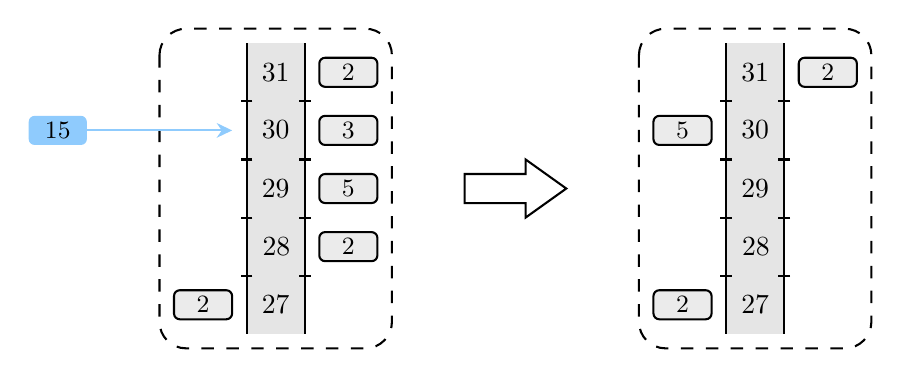
\begin{tikzpicture}[x=0.75pt,y=0.75pt,yscale=-0.7,xscale=0.7]
%uncomment if require: \path (0,300); %set diagram left start at 0, and has height of 300


%Shape: Rectangle [id:dp8412452715917856] 
\draw  [draw opacity=0][fill={rgb, 255:red, 0; green, 0; blue, 0 }  ,fill opacity=0.1 ] (190,50) -- (230,50) -- (230,250) -- (190,250) -- cycle ;
%Rounded Rect [id:dp007986415015731718] 
\draw  [fill={rgb, 255:red, 235; green, 235; blue, 235 }  ,fill opacity=1 ][line width=0.75]  (240,144) .. controls (240,141.79) and (241.79,140) .. (244,140) -- (276,140) .. controls (278.21,140) and (280,141.79) .. (280,144) -- (280,156) .. controls (280,158.21) and (278.21,160) .. (276,160) -- (244,160) .. controls (241.79,160) and (240,158.21) .. (240,156) -- cycle ;
%Straight Lines [id:da2293722746628727] 
\draw    (190,50) -- (190,250) (194,90) -- (186,90)(194,130) -- (186,130)(194,170) -- (186,170)(194,210) -- (186,210) ;
%Straight Lines [id:da3120213615797991] 
\draw    (230,50) -- (230,250) (234,90) -- (226,90)(234,130) -- (226,130)(234,170) -- (226,170)(234,210) -- (226,210) ;
%Rounded Rect [id:dp10621428282249978] 
\draw  [fill={rgb, 255:red, 235; green, 235; blue, 235 }  ,fill opacity=1 ][line width=0.75]  (240,104) .. controls (240,101.79) and (241.79,100) .. (244,100) -- (276,100) .. controls (278.21,100) and (280,101.79) .. (280,104) -- (280,116) .. controls (280,118.21) and (278.21,120) .. (276,120) -- (244,120) .. controls (241.79,120) and (240,118.21) .. (240,116) -- cycle ;
%Rounded Rect [id:dp03800501182586913] 
\draw  [fill={rgb, 255:red, 235; green, 235; blue, 235 }  ,fill opacity=1 ][line width=0.75]  (140,224) .. controls (140,221.79) and (141.79,220) .. (144,220) -- (176,220) .. controls (178.21,220) and (180,221.79) .. (180,224) -- (180,236) .. controls (180,238.21) and (178.21,240) .. (176,240) -- (144,240) .. controls (141.79,240) and (140,238.21) .. (140,236) -- cycle ;
%Rounded Rect [id:dp3338924127776648] 
\draw  [dash pattern={on 4.5pt off 4.5pt}] (130,58.3) .. controls (130,48.19) and (138.19,40) .. (148.3,40) -- (271.7,40) .. controls (281.81,40) and (290,48.19) .. (290,58.3) -- (290,241.7) .. controls (290,251.81) and (281.81,260) .. (271.7,260) -- (148.3,260) .. controls (138.19,260) and (130,251.81) .. (130,241.7) -- cycle ;
%Rounded Rect [id:dp38799186795833285] 
\draw  [fill={rgb, 255:red, 235; green, 235; blue, 235 }  ,fill opacity=1 ][line width=0.75]  (240,64) .. controls (240,61.79) and (241.79,60) .. (244,60) -- (276,60) .. controls (278.21,60) and (280,61.79) .. (280,64) -- (280,76) .. controls (280,78.21) and (278.21,80) .. (276,80) -- (244,80) .. controls (241.79,80) and (240,78.21) .. (240,76) -- cycle ;
%Rounded Rect [id:dp932038680993432] 
\draw  [draw opacity=0][fill={rgb, 255:red, 143; green, 203; blue, 253 }  ,fill opacity=1 ][dash pattern={on 4.5pt off 4.5pt}][line width=0.75]  (40,104) .. controls (40,101.79) and (41.79,100) .. (44,100) -- (76,100) .. controls (78.21,100) and (80,101.79) .. (80,104) -- (80,116) .. controls (80,118.21) and (78.21,120) .. (76,120) -- (44,120) .. controls (41.79,120) and (40,118.21) .. (40,116) -- cycle ;
%Straight Lines [id:da1966192901653835] 
\draw [color={rgb, 255:red, 143; green, 203; blue, 253 }  ,draw opacity=1 ]   (80,110) -- (177,110) ;
\draw [shift={(180,110)}, rotate = 180] [fill={rgb, 255:red, 143; green, 203; blue, 253 }  ,fill opacity=1 ][line width=0.08]  [draw opacity=0] (10.72,-5.15) -- (0,0) -- (10.72,5.15) -- (7.12,0) -- cycle    ;
%Shape: Rectangle [id:dp20325610013103357] 
\draw  [draw opacity=0][fill={rgb, 255:red, 0; green, 0; blue, 0 }  ,fill opacity=0.1 ] (520,50) -- (560,50) -- (560,250) -- (520,250) -- cycle ;
%Rounded Rect [id:dp24083299793098112] 
\draw  [fill={rgb, 255:red, 235; green, 235; blue, 235 }  ,fill opacity=1 ][line width=0.75]  (470,104) .. controls (470,101.79) and (471.79,100) .. (474,100) -- (506,100) .. controls (508.21,100) and (510,101.79) .. (510,104) -- (510,116) .. controls (510,118.21) and (508.21,120) .. (506,120) -- (474,120) .. controls (471.79,120) and (470,118.21) .. (470,116) -- cycle ;
%Straight Lines [id:da7915001823532407] 
\draw    (520,50) -- (520,250) (524,90) -- (516,90)(524,130) -- (516,130)(524,170) -- (516,170)(524,210) -- (516,210) ;
%Straight Lines [id:da9500452904072452] 
\draw    (560,50) -- (560,250) (564,90) -- (556,90)(564,130) -- (556,130)(564,170) -- (556,170)(564,210) -- (556,210) ;
%Rounded Rect [id:dp31551226522886167] 
\draw  [fill={rgb, 255:red, 235; green, 235; blue, 235 }  ,fill opacity=1 ][line width=0.75]  (470,224) .. controls (470,221.79) and (471.79,220) .. (474,220) -- (506,220) .. controls (508.21,220) and (510,221.79) .. (510,224) -- (510,236) .. controls (510,238.21) and (508.21,240) .. (506,240) -- (474,240) .. controls (471.79,240) and (470,238.21) .. (470,236) -- cycle ;
%Rounded Rect [id:dp14842743068542508] 
\draw  [dash pattern={on 4.5pt off 4.5pt}] (460,58.3) .. controls (460,48.19) and (468.19,40) .. (478.3,40) -- (601.7,40) .. controls (611.81,40) and (620,48.19) .. (620,58.3) -- (620,241.7) .. controls (620,251.81) and (611.81,260) .. (601.7,260) -- (478.3,260) .. controls (468.19,260) and (460,251.81) .. (460,241.7) -- cycle ;
%Rounded Rect [id:dp13336948832097884] 
\draw  [fill={rgb, 255:red, 235; green, 235; blue, 235 }  ,fill opacity=1 ][line width=0.75]  (570,64) .. controls (570,61.79) and (571.79,60) .. (574,60) -- (606,60) .. controls (608.21,60) and (610,61.79) .. (610,64) -- (610,76) .. controls (610,78.21) and (608.21,80) .. (606,80) -- (574,80) .. controls (571.79,80) and (570,78.21) .. (570,76) -- cycle ;
%Rounded Rect [id:dp3708973876475854] 
\draw  [fill={rgb, 255:red, 235; green, 235; blue, 235 }  ,fill opacity=1 ][line width=0.75]  (240,184) .. controls (240,181.79) and (241.79,180) .. (244,180) -- (276,180) .. controls (278.21,180) and (280,181.79) .. (280,184) -- (280,196) .. controls (280,198.21) and (278.21,200) .. (276,200) -- (244,200) .. controls (241.79,200) and (240,198.21) .. (240,196) -- cycle ;
%Right Arrow [id:dp26035875111685947] 
\draw   (340,140) -- (382,140) -- (382,130) -- (410,150) -- (382,170) -- (382,160) -- (340,160) -- cycle ;

% Text Node
\draw (210,70) node    {$31$};
% Text Node
\draw (210,109.5) node    {$30$};
% Text Node
\draw (260,150) node  [font=\small]  {$5$};
% Text Node
\draw (210,150) node    {$29$};
% Text Node
\draw (210.5,190) node    {$28$};
% Text Node
\draw (210,230) node    {$27$};
% Text Node
\draw (260,110) node  [font=\small]  {$3$};
% Text Node
\draw (160,230) node  [font=\small]  {$2$};
% Text Node
\draw (260,70) node  [font=\small]  {$2$};
% Text Node
\draw (60,110) node  [font=\small]  {$15$};
% Text Node
\draw (540,70) node    {$31$};
% Text Node
\draw (540,109.5) node    {$30$};
% Text Node
\draw (490,110) node  [font=\small]  {$5$};
% Text Node
\draw (540,150) node    {$29$};
% Text Node
\draw (540.5,190) node    {$28$};
% Text Node
\draw (540,230) node    {$27$};
% Text Node
\draw (490,230) node  [font=\small]  {$2$};
% Text Node
\draw (590,70) node  [font=\small]  {$2$};
% Text Node
\draw (260,190) node  [font=\small]  {$2$};


\end{tikzpicture}

  \end{center}
\end{frame}

\begin{frame}{Limit Orderbook Examples}
  \begin{columns}[T]
    \begin{column}{0.4\textwidth}
      

\tikzset{every picture/.style={line width=0.75pt}} %set default line width to 0.75pt        

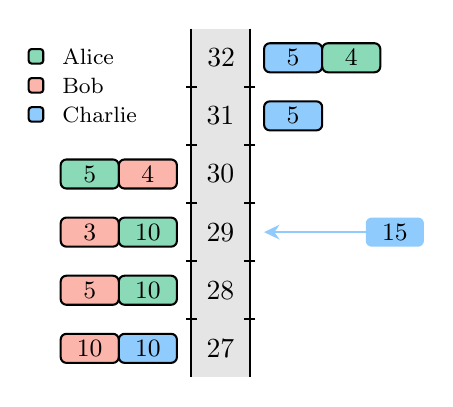
\begin{tikzpicture}[x=0.75pt,y=0.75pt,yscale=-0.7,xscale=0.7]
%uncomment if require: \path (0,300); %set diagram left start at 0, and has height of 300

%Shape: Rectangle [id:dp5750504893681659] 
\draw  [draw opacity=0][fill={rgb, 255:red, 0; green, 0; blue, 0 }  ,fill opacity=0.1 ] (140,30) -- (180,30) -- (180,270) -- (140,270) -- cycle ;
%Rounded Rect [id:dp6877205326451323] 
\draw  [fill={rgb, 255:red, 138; green, 218; blue, 184 }  ,fill opacity=1 ][line width=0.75]  (50,124) .. controls (50,121.79) and (51.79,120) .. (54,120) -- (86,120) .. controls (88.21,120) and (90,121.79) .. (90,124) -- (90,136) .. controls (90,138.21) and (88.21,140) .. (86,140) -- (54,140) .. controls (51.79,140) and (50,138.21) .. (50,136) -- cycle ;
%Straight Lines [id:da215961151995397] 
\draw    (140,30) -- (140,270) (144,70) -- (136,70)(144,110) -- (136,110)(144,150) -- (136,150)(144,190) -- (136,190)(144,230) -- (136,230) ;
%Straight Lines [id:da620143052535216] 
\draw    (180,30) -- (180,270) (184,70) -- (176,70)(184,110) -- (176,110)(184,150) -- (176,150)(184,190) -- (176,190)(184,230) -- (176,230) ;
%Rounded Rect [id:dp9487758453323831] 
\draw  [fill={rgb, 255:red, 251; green, 181; blue, 170 }  ,fill opacity=1 ][line width=0.75]  (50,164) .. controls (50,161.79) and (51.79,160) .. (54,160) -- (86,160) .. controls (88.21,160) and (90,161.79) .. (90,164) -- (90,176) .. controls (90,178.21) and (88.21,180) .. (86,180) -- (54,180) .. controls (51.79,180) and (50,178.21) .. (50,176) -- cycle ;
%Rounded Rect [id:dp2348115833646376] 
\draw  [fill={rgb, 255:red, 138; green, 218; blue, 184 }  ,fill opacity=1 ][line width=0.75]  (90,164) .. controls (90,161.79) and (91.79,160) .. (94,160) -- (126,160) .. controls (128.21,160) and (130,161.79) .. (130,164) -- (130,176) .. controls (130,178.21) and (128.21,180) .. (126,180) -- (94,180) .. controls (91.79,180) and (90,178.21) .. (90,176) -- cycle ;
%Rounded Rect [id:dp2584842224306618] 
\draw  [fill={rgb, 255:red, 138; green, 218; blue, 184 }  ,fill opacity=1 ][line width=0.75]  (90,204) .. controls (90,201.79) and (91.79,200) .. (94,200) -- (126,200) .. controls (128.21,200) and (130,201.79) .. (130,204) -- (130,216) .. controls (130,218.21) and (128.21,220) .. (126,220) -- (94,220) .. controls (91.79,220) and (90,218.21) .. (90,216) -- cycle ;
%Rounded Rect [id:dp05087451015493316] 
\draw  [fill={rgb, 255:red, 251; green, 181; blue, 170 }  ,fill opacity=1 ][line width=0.75]  (50,204) .. controls (50,201.79) and (51.79,200) .. (54,200) -- (86,200) .. controls (88.21,200) and (90,201.79) .. (90,204) -- (90,216) .. controls (90,218.21) and (88.21,220) .. (86,220) -- (54,220) .. controls (51.79,220) and (50,218.21) .. (50,216) -- cycle ;
%Rounded Rect [id:dp9710519793908792] 
\draw  [fill={rgb, 255:red, 251; green, 181; blue, 170 }  ,fill opacity=1 ][line width=0.75]  (50,244) .. controls (50,241.79) and (51.79,240) .. (54,240) -- (86,240) .. controls (88.21,240) and (90,241.79) .. (90,244) -- (90,256) .. controls (90,258.21) and (88.21,260) .. (86,260) -- (54,260) .. controls (51.79,260) and (50,258.21) .. (50,256) -- cycle ;
%Rounded Rect [id:dp7721373725752443] 
\draw  [fill={rgb, 255:red, 138; green, 218; blue, 184 }  ,fill opacity=1 ][line width=0.75]  (28,46) .. controls (28,44.9) and (28.9,44) .. (30,44) -- (36,44) .. controls (37.1,44) and (38,44.9) .. (38,46) -- (38,52) .. controls (38,53.1) and (37.1,54) .. (36,54) -- (30,54) .. controls (28.9,54) and (28,53.1) .. (28,52) -- cycle ;
%Rounded Rect [id:dp4648823353022742] 
\draw  [fill={rgb, 255:red, 143; green, 203; blue, 253 }  ,fill opacity=1 ][line width=0.75]  (28,86) .. controls (28,84.9) and (28.9,84) .. (30,84) -- (36,84) .. controls (37.1,84) and (38,84.9) .. (38,86) -- (38,92) .. controls (38,93.1) and (37.1,94) .. (36,94) -- (30,94) .. controls (28.9,94) and (28,93.1) .. (28,92) -- cycle ;
%Rounded Rect [id:dp396175075326069] 
\draw  [fill={rgb, 255:red, 251; green, 181; blue, 170 }  ,fill opacity=1 ][line width=0.75]  (28,66) .. controls (28,64.9) and (28.9,64) .. (30,64) -- (36,64) .. controls (37.1,64) and (38,64.9) .. (38,66) -- (38,72) .. controls (38,73.1) and (37.1,74) .. (36,74) -- (30,74) .. controls (28.9,74) and (28,73.1) .. (28,72) -- cycle ;
%Rounded Rect [id:dp10932219999579096] 
\draw  [fill={rgb, 255:red, 143; green, 203; blue, 253 }  ,fill opacity=1 ][line width=0.75]  (190,44) .. controls (190,41.79) and (191.79,40) .. (194,40) -- (226,40) .. controls (228.21,40) and (230,41.79) .. (230,44) -- (230,56) .. controls (230,58.21) and (228.21,60) .. (226,60) -- (194,60) .. controls (191.79,60) and (190,58.21) .. (190,56) -- cycle ;
%Rounded Rect [id:dp9836145210038129] 
\draw  [fill={rgb, 255:red, 143; green, 203; blue, 253 }  ,fill opacity=1 ][line width=0.75]  (90,244) .. controls (90,241.79) and (91.79,240) .. (94,240) -- (126,240) .. controls (128.21,240) and (130,241.79) .. (130,244) -- (130,256) .. controls (130,258.21) and (128.21,260) .. (126,260) -- (94,260) .. controls (91.79,260) and (90,258.21) .. (90,256) -- cycle ;
%Rounded Rect [id:dp5732951285894992] 
\draw  [fill={rgb, 255:red, 138; green, 218; blue, 184 }  ,fill opacity=1 ][line width=0.75]  (230,44) .. controls (230,41.79) and (231.79,40) .. (234,40) -- (266,40) .. controls (268.21,40) and (270,41.79) .. (270,44) -- (270,56) .. controls (270,58.21) and (268.21,60) .. (266,60) -- (234,60) .. controls (231.79,60) and (230,58.21) .. (230,56) -- cycle ;
%Straight Lines [id:da15472498021828307] 
\draw [color={rgb, 255:red, 143; green, 203; blue, 253 }  ,draw opacity=1 ]   (260,170) -- (193,170) ;
\draw [shift={(190,170)}, rotate = 360] [fill={rgb, 255:red, 143; green, 203; blue, 253 }  ,fill opacity=1 ][line width=0.08]  [draw opacity=0] (10.72,-5.15) -- (0,0) -- (10.72,5.15) -- (7.12,0) -- cycle    ;
%Rounded Rect [id:dp20817918206073804] 
\draw  [draw opacity=0][fill={rgb, 255:red, 143; green, 203; blue, 253 }  ,fill opacity=1 ][dash pattern={on 4.5pt off 4.5pt}][line width=0.75]  (260,164) .. controls (260,161.79) and (261.79,160) .. (264,160) -- (296,160) .. controls (298.21,160) and (300,161.79) .. (300,164) -- (300,176) .. controls (300,178.21) and (298.21,180) .. (296,180) -- (264,180) .. controls (261.79,180) and (260,178.21) .. (260,176) -- cycle ;
%Rounded Rect [id:dp8342306342416866] 
\draw  [fill={rgb, 255:red, 251; green, 181; blue, 170 }  ,fill opacity=1 ][line width=0.75]  (90,124) .. controls (90,121.79) and (91.79,120) .. (94,120) -- (126,120) .. controls (128.21,120) and (130,121.79) .. (130,124) -- (130,136) .. controls (130,138.21) and (128.21,140) .. (126,140) -- (94,140) .. controls (91.79,140) and (90,138.21) .. (90,136) -- cycle ;
%Rounded Rect [id:dp39224731910080646] 
\draw  [fill={rgb, 255:red, 143; green, 203; blue, 253 }  ,fill opacity=1 ][line width=0.75]  (190,84) .. controls (190,81.79) and (191.79,80) .. (194,80) -- (226,80) .. controls (228.21,80) and (230,81.79) .. (230,84) -- (230,96) .. controls (230,98.21) and (228.21,100) .. (226,100) -- (194,100) .. controls (191.79,100) and (190,98.21) .. (190,96) -- cycle ;

% Text Node
\draw (160,90) node    {$31$};
% Text Node
\draw (160,129.5) node    {$30$};
% Text Node
\draw (70,130) node  [font=\small]  {${\textstyle 5}$};
% Text Node
\draw (160,170) node    {$29$};
% Text Node
\draw (160,210) node    {$28$};
% Text Node
\draw (160,250) node    {$27$};
% Text Node
\draw (70,170) node  [font=\small]  {$3$};
% Text Node
\draw (110,170) node  [font=\small]  {$10$};
% Text Node
\draw (110,210) node  [font=\small]  {$10$};
% Text Node
\draw (70,210) node  [font=\small]  {${\textstyle 5}$};
% Text Node
\draw (70,250) node  [font=\small]  {$10$};
% Text Node
\draw (49,42) node [anchor=north west][inner sep=0.75pt]  [font=\footnotesize] [align=left] {Alice};
% Text Node
\draw (49,62) node [anchor=north west][inner sep=0.75pt]  [font=\footnotesize] [align=left] {Bob};
% Text Node
\draw (49,82) node [anchor=north west][inner sep=0.75pt]  [font=\footnotesize] [align=left] {Charlie};
% Text Node
\draw (160.5,50) node    {$32$};
% Text Node
\draw (210,50) node  [font=\small]  {$5$};
% Text Node
\draw (110,250) node  [font=\small]  {$10$};
% Text Node
\draw (250,50) node  [font=\small]  {$4$};
% Text Node
\draw (280,170) node  [font=\small]  {$15$};
% Text Node
\draw (110,130) node  [font=\small]  {$4$};
% Text Node
\draw (210,90) node  [font=\small]  {$5$};


\end{tikzpicture}

    \end{column}

    \begin{column}{0.6\textwidth}
      \textbf{Discussion Questions}
      \begin{itemize}
        \item What trades are made when Charlie inserts the offer?
        \item How does each person's position change?
        \item What does the orderbook look like afterwards?
        \item How does Charlie's opinion differ from Alice's and Bob's?
      \end{itemize}
    \end{column}
  \end{columns}

\end{frame}
